\section{Évaluation de l'hypothèse d'efficience}
\label{section:4.2-HYPOTHESE-EFFICIENCE}
% « \textit{quels sont les paramètres optimaux pour minimiser la charge de travail de l'annotateur ?} »

	%%% Formulation des hypothèses:
	Suite à la validation de l'hypothèse d'efficacité (convergence de la méthode, cf. section~\ref{section:4.1-HYPOTHESE-EFFICACITE}), nous aimerions vérifier l'hypothèse suivante :

	\begin{tcolorbox}[
		title=\faVial~\textbf{Hypothèse d'efficience}~\faVial,
		colback=colorTcolorboxHypothesis!15,
		colframe=colorTcolorboxHypothesis!75,
		width=\linewidth
	]

		% Hypothèse.
		« \textbf{
			La vitesse de convergence du \textit{clustering} interactif peut être optimisée en ajustant différents paramètres afin de minimiser la charge de travail de l'opérateur. Nous étudierons en particulier l'influence du prétraitement des données, de la vectorisation des données, de l'échantillonnage des contraintes à annoter et du \textit{clustering} sous contraintes.
		} » \\
		
		% Résumé de l'étude.
		Afin de vérifier cette hypothèse, nous mettrons en place une expérience de ré-annotation d'une base d'apprentissage (qui servira ici de vérité terrain) à l'aide de notre méthode, en simulant l'annotation d'un expert, et nous réaliserons l'analyse statistique de la taille d'effet de différents paramètres sur la vitesse de convergence du \textit{clustering} itératif.
		
		% Figure.
		La figure~\ref{figure:4.2-HYPOTHESE-EFFICIENCE} illustre cette hypothèse et l'espoir d'une convergence "optimale" d'une base d'apprentissage en cours de construction vers sa vérité terrain.
		%
		\begin{figure}[H]  % keep [H] to be in the tcolorbox.
			\centering
			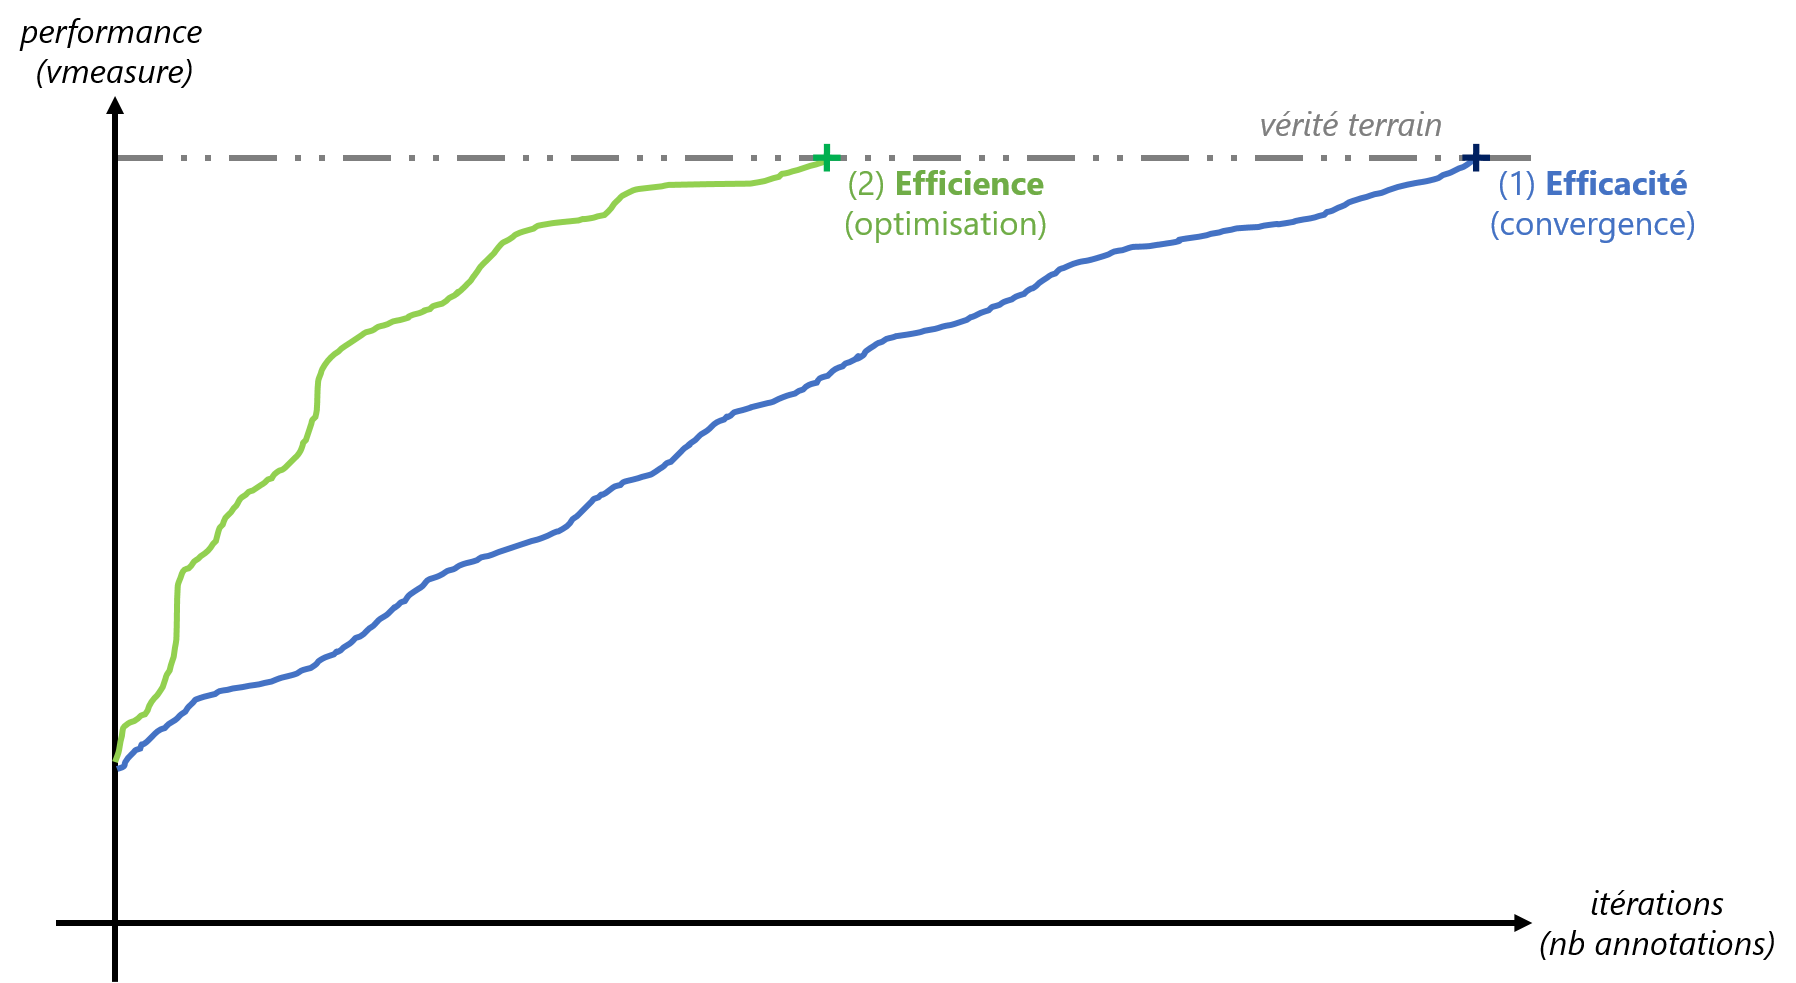
\includegraphics[width=0.8\textwidth]{figures/hypotheses-02-efficience}
			\caption{Illustration des études réalisées sur le \textit{clustering} interactif (\textit{étape 2/6}) en schématisant l'évolution de la performance (\textit{accord avec la vérité terrain calculé en v-measure}) d'une base d'apprentissage en cours de construction en fonction du nombre d'itérations de la méthode (\textit{nombre d'annotations par un expert métier}).}
			\label{figure:4.2-HYPOTHESE-EFFICIENCE}
		\end{figure}

	\end{tcolorbox}
	
	%%%
	%%% Subsection 4.2.1: Étude d'optimisation des paramètres de convergence.
	%%%
	\subsection{Étude d'optimisation des paramètres de convergence}
	\label{subsection:4.2.1-ETUDE-OPTIMISATION}
			
		% Référence articles.
		\begin{leftBarInformation}
			Cette étude a été l'objet d'une présentation à la conférence \texttt{EGC (Extraction et Gestion des Connaissances)}~\citep{schild:conception-interactive-clustering:2021}, et d'une extension dans le journal \texttt{IJDWM (International Journal of Data Warehousing and Mining)}~\citep{schild:extension-interactive-clustering:2022}.
			\footnote{Les résultats et la discussion ont été mis à jour et réécrits pour mieux s'intégrer au discours ce manuscrit.}
		\end{leftBarInformation}

		%%% Protocole expérimental.
		\subsubsection{Protocole expérimental : analyser la taille d'effet paramètres sur la vitesse de création d'une base d'apprentissage}

			% Objectif de l'expérience.
			Nous voulons étudier l'influence des paramètres de notre implémentation du \textit{clustering} interactif sur la vitesse de création d'une base d'apprentissage pour un assistant conversationnel.
			Pour cette étude, nous allons reprendre le protocole expérimental de l'étude de convergence en section~\ref{subsection:4.1.1-ETUDE-CONVERGENCE} visant à simuler la création d'une base d'apprentissage\todo{référence, lien vers ANNEXE}.
			
			% Détails de l'expérience.
			En s'appuyant sur les résultats précédemment obtenus, nous allons analyser l'influence des différentes tâches employées (\textbf{prétraitement}, \textbf{vectorisation}, \textbf{clustering sous contraintes}, \textbf{échantillonnage}) et de leurs paramètres sur la vitesse de convergence vers la vérité terrain.
			% Description implémentation de l'interactive clustering.
			Nous avons toujours \texttt{192} combinaisons testées, et chaque tentative est répétée \texttt{5} fois pour contrer les aléas statistiques de certains algorithmes.
			Pour plus de détails sur ces algorithmes, référez-vous à la section~\ref{section:3.3-DESCRIPTION-IMPLEMENTATION}.
			
			% Description de l'évaluation et Seuils d'évaluation.
			Comme lors de l'étude sur la convergence de la méthode, nous nous intéresserons à l'évolution de la \texttt{v-measure} entre la vérité terrain et notre segmentation des données obtenue, et nous affinerons notre évaluation en portant attention aux trois seuils d'annotations suivants :
			\begin{enumerate}
				\item le cas d'une \textbf{annotation partielle}, correspondant au nombre d'itérations nécessaires à la méthode pour avoir \texttt{90}\% de \texttt{v-measure} entre le résultat obtenu et la vérité terrain, c'est-à-dire un état de semi-parcours vers une convergence totale\footnote{Le seuil de \texttt{90}\% a été choisi au cours de l'étude de convergence (cf. hypothèse d'efficacité, section~\ref{section:4.1-HYPOTHESE-EFFICACITE}).} ;
				\item le cas d'une \textbf{annotation suffisante}, correspondant au nombre d'itérations nécessaires à la méthode pour avoir \texttt{100}\% de \texttt{v-measure} entre le résultat obtenu et la vérité terrain, c'est-à-dire avoir suffisamment de contraintes annotées par l'expert métier pour retrouver la vérité terrain ;
				\item le cas d'une \textbf{annotation exhaustive}, correspondant au nombre d'itérations nécessaires à la méthode pour parcourir toutes les contraintes possibles sur les données, et ainsi retranscrire exhaustivement la vision de l'expert métier.
			\end{enumerate}
			
			% Description de l'analyse ANOVA.
			Enfin, nous utiliserons une \texttt{ANOVA} à mesures répétées afin de déterminer l’effet des paramètres de notre implémentation sur le nombre d’annotations requis pour converger vers la vérité terrain. Ces analyses seront réalisées à l'aide du logiciel R\todo{citation}, et le test de \texttt{Tukey (HSD)} est utilisé pour les comparaisons post-hoc.
			
			% Pseudo-code.
			Pour résumer ce protocole expérimental, vous pouvez vous référez au pseudo-code décrit dans Alg.~\ref{algorithm:4.2.1-ETUDE-OPTIMISATION-PROTOCOLE}.
			%
			\begin{algorithm}[!htb]
				\begin{algorithmic}[1]
					\Require jeu de données annoté (vérité terrain)
					\ForAll{arrangement d'algorithmes et de paramètres à tester}
						\State \textbf{initialisation}: récupérer les données de la vérité terrain sans leur label, créer une liste vide de contraintes
						\State \textbf{prétraitement}: supprimer le bruit dans les données
						\State \textbf{vectorisation}: transformer les données en vecteurs
						\State \textbf{clustering initial}: regrouper les données par similarité
						\State \textbf{évaluation}: estimer l'équivalence entre le clustering obtenu et la vérité terrain
						\Repeat
							\State \textbf{échantillonnage}: sélectionner de nouvelles contraintes à annoter
							\State \textbf{simulation d'annotation}: ajouter des contraintes grâce à la comparaison des labels de la vérité terrain
							\State \textbf{clustering}: regrouper les données par similarité avec les contraintes
							\State \textbf{évaluation}: estimer l'équivalence entre le clustering obtenu et la vérité terrain
						\Until{annotation de toutes les contraintes possibles}
					\EndFor
					\State \textbf{analyse}: déterminer les tailles d'effets des algorithmes et paramètres
					\Ensure meilleurs arrangements d'algorithmes et de paramètres
				\end{algorithmic}
				\caption{Description en pseudo-code du protocole expérimental de l'étude d'optimisation de la convergence du \textit{clustering} interactif vers une vérité terrain pré-établie.}
				\label{algorithm:4.2.1-ETUDE-OPTIMISATION-PROTOCOLE}
			\end{algorithm}
			
			% Référence scripts.
			\begin{leftBarInformation}
				Les scripts de l'expérience (\textit{notebooks} Python) sont disponibles dans un dossier dédié de~\cite{schild:cognitivefactory-interactive-clustering-comparative-study:2021}.
			\end{leftBarInformation}

		%%% Résultats
		\subsubsection{Résultats obtenus}
		
			% Analyse d'une annotation partielle.
			Pour obtenir une \textbf{annotation partielle} (\textit{atteindre une \texttt{v-measure} de \texttt{90}\%}), la moyenne des itérations est de \texttt{59.04} (min: \texttt{11}, max: \texttt{315}, écart-type: \texttt{42.14}), soit une moyenne de \texttt{2 951.81} annotations (min: \texttt{550}, max: \texttt{15 750}, écart-type: \texttt{2 106.72}).
			La figure~\ref{figure:4.2.1-ETUDE-OPTIMISATION-HISTOGRAMME-ANNOTATION-PARTIELLE} représente la répartition de ces itérations au cours des différentes tentatives.
			On peut noter les deux cas intéressants suivants :
			%
			\begin{itemize}
				\item[\(\bullet\)] Les tentatives les plus rapides furent celles avec un prétraitement des données \texttt{prep.no} ou \texttt{prep.simple} ou \texttt{prep.lemma}, une vectorisation des données \texttt{vect.tfidf}, un clustering sous contraintes \texttt{clust.hier.sing}, et un échantillonnage de contraintes \texttt{samp.closest.diff}. Ces tentatives ont requis \texttt{11} itérations, soit \texttt{550} annotations, dont \texttt{299} (respectivement \texttt{304} et \texttt{281}) contraintes \texttt{MUST-LINK}.
				\item[\(\bullet\)] Les tentatives les plus lentes furent celles avec un prétraitement des données \texttt{prep.no}, une vectorisation des données \texttt{vect.tfidf}, un clustering sous contraintes \texttt{clust.spec}, et un échantillonnage de contraintes \texttt{samp.farthest.same}. Ces tentatives ont requis \texttt{315} itérations, soit \texttt{15 750} annotations, dont \texttt{1 032} contraintes \texttt{MUST-LINK}.
			\end{itemize}
			%
			\begin{figure}[!htb]
				\centering
				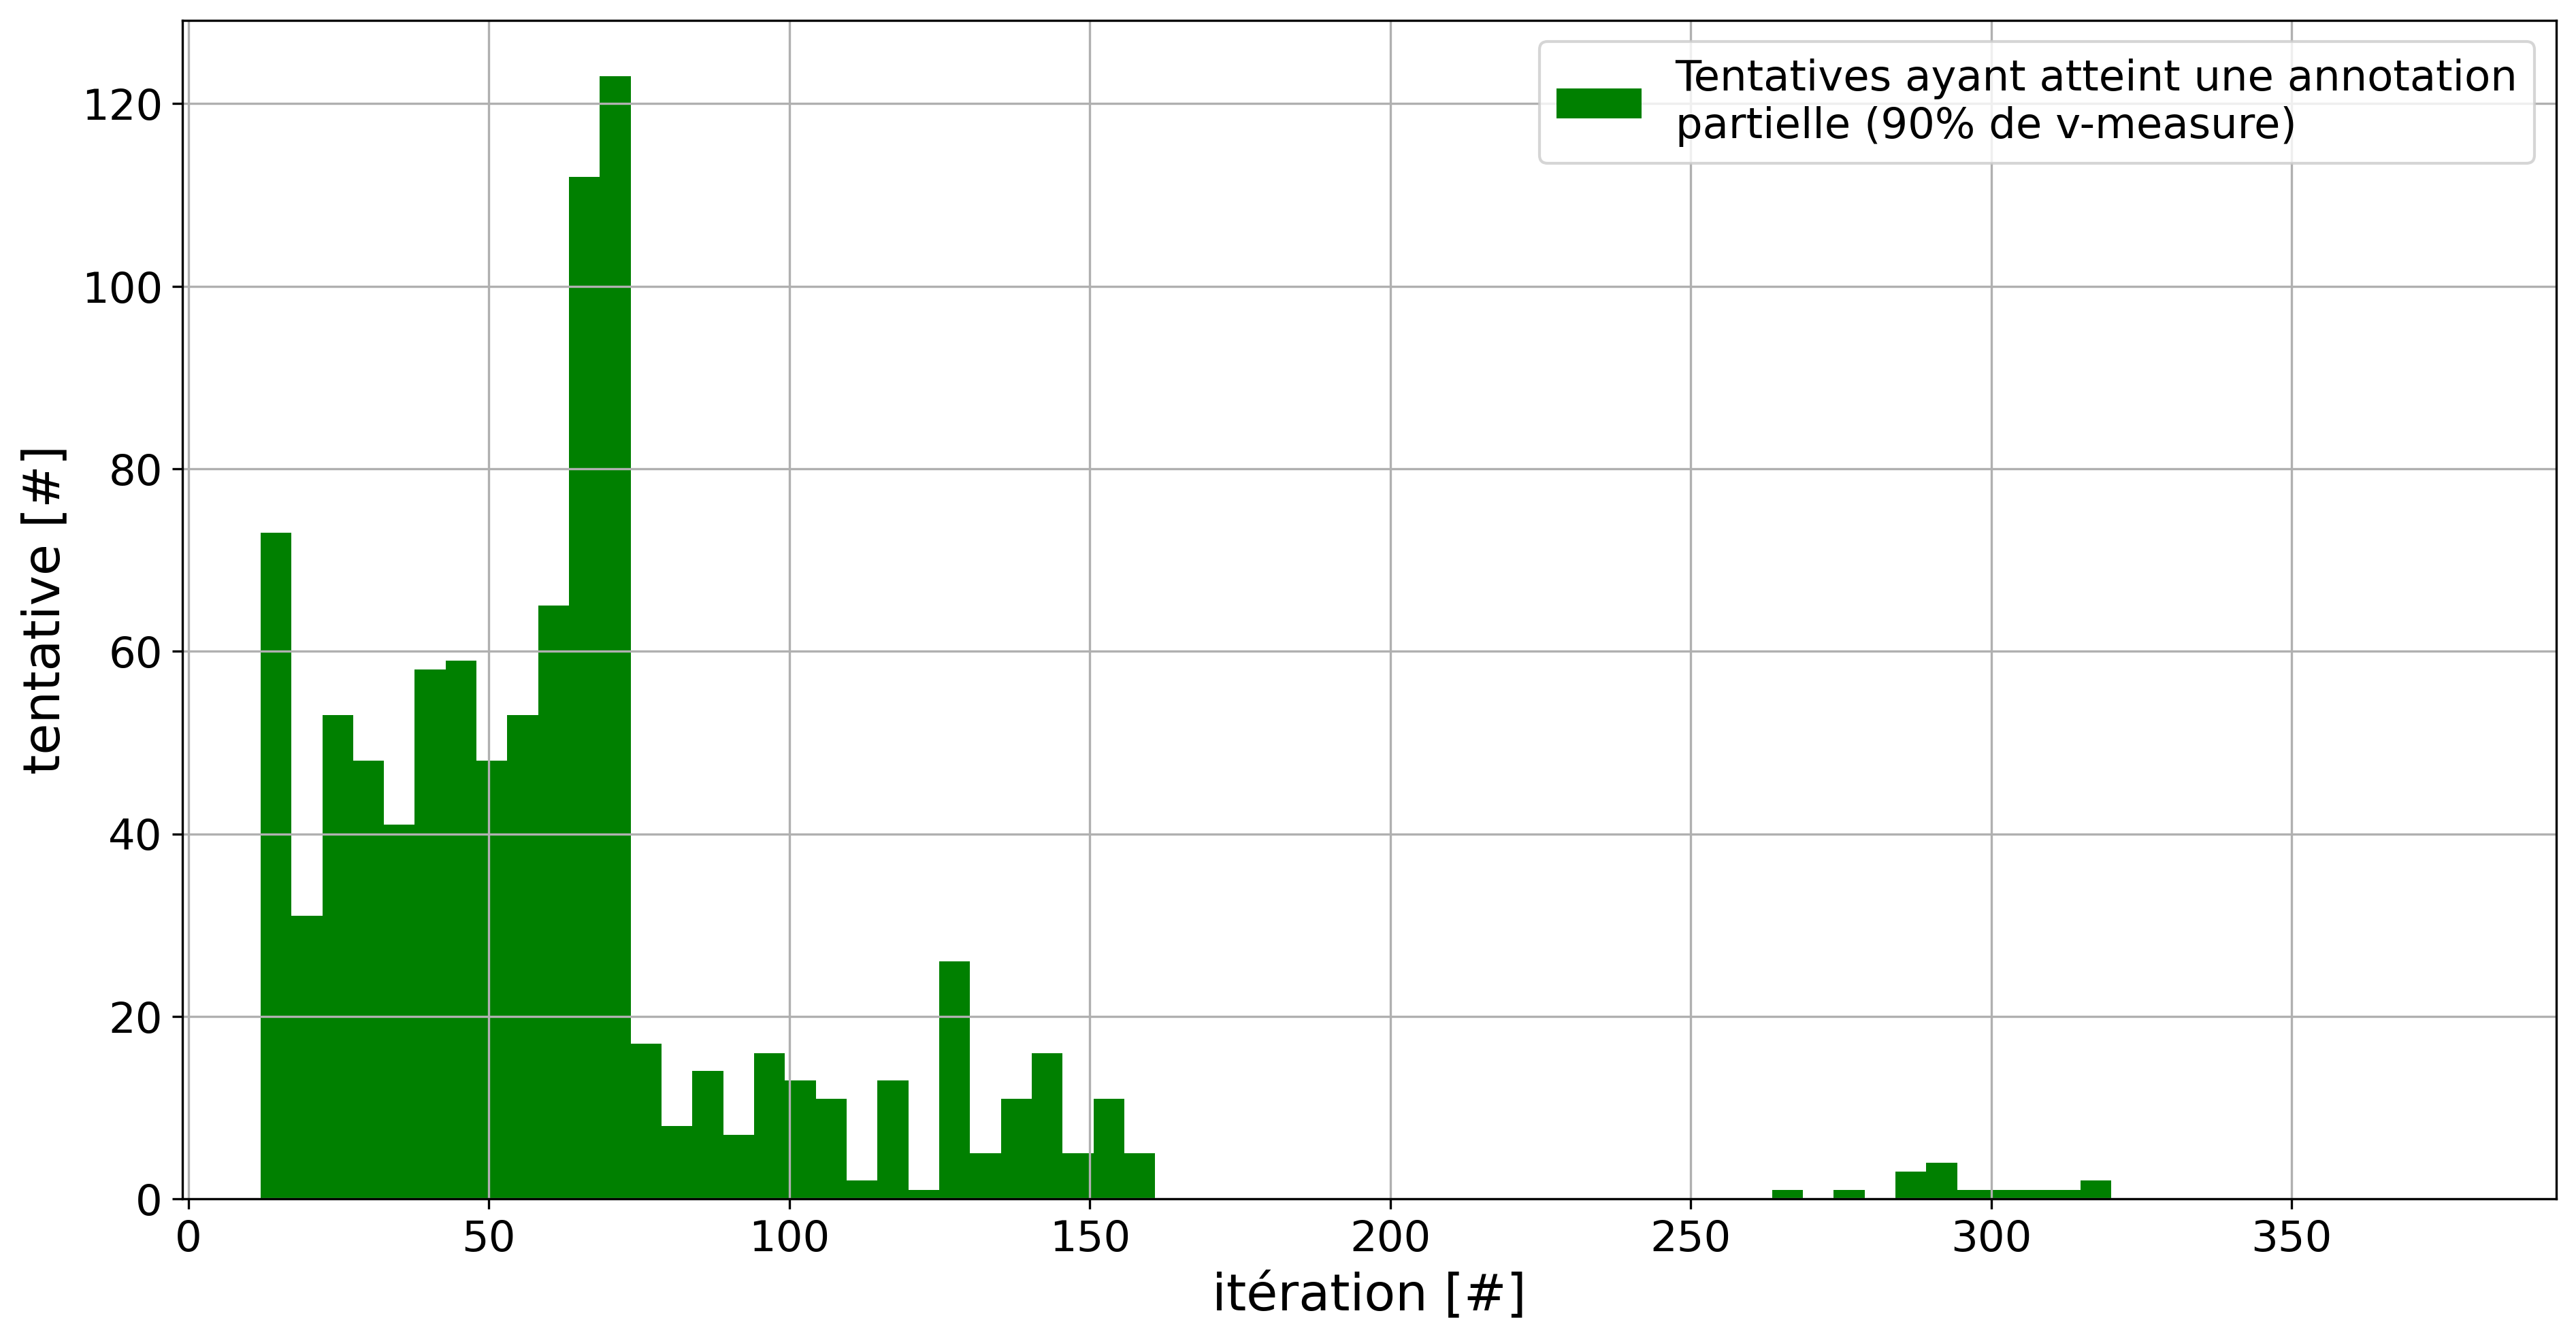
\includegraphics[width=0.7\textwidth]{figures/etude-efficience-histogramme-annotation-partielle}
				\caption{Répartition des tentatives en fonction de l'itération de la méthode à laquelle elles atteignent le seuil d'une annotation partielle, c'est-à-dire l'itération à laquelle elles parviennent à \texttt{90}\% de \texttt{v-measure} entre un résultat obtenu et la vérité terrain. L'histogramme est réduit à \texttt{60} pics pour simplifier l'affichage.}
				\label{figure:4.2.1-ETUDE-OPTIMISATION-HISTOGRAMME-ANNOTATION-PARTIELLE}
			\end{figure}
			%
			Le tableau~\ref{table:4.2.1-ETUDE-OPTIMISATION-ANOVA-ANNOTATION-PARTIELLE} retranscrit l'influence de chacun des paramètres sur le nombre d'itérations nécessaires pour atteindre une \textbf{annotation partielle} (\textit{atteindre une \texttt{v-measure} de \texttt{90}\%}).
			Les analyses de variance mettent en relief l'effet significatif sur cette convergence du prétraitement (eta-carré: \texttt{0.320}, p-valeur: \(<\) \texttt{\(10^{-3}\)}), de la vectorisation (eta-carré: \texttt{0.388}, p-valeur: \(<\) \texttt{\(10^{-3}\)}), du clustering (eta-carré: \texttt{0.866}, p-valeur: \(<\) \texttt{\(10^{-3}\)}) et de l'échantillonnage (eta-carré: \texttt{0.968}, p-valeur: \(<\) \texttt{\(10^{-3}\)}).
			L'analyse post-hoc de ces effets indique que le meilleur paramétrage moyen pour atteindre une \textbf{annotation partielle} repose sur la prétraitement \texttt{prep.simple}, le vectorisation \texttt{vect.tfidf}, le clustering \texttt{clust.hier.avg}, et l'échantillonnage \texttt{samp.closest.diff}. La moyenne du nombre d'itération requis pour ce paramétrage est de \texttt{19.00} (écart-type: \texttt{0.79}), soit \texttt{950} annotations (écart-type: \texttt{39.34}).
			%
			\begin{table}[!htb]
				\begin{center}
				\begin{tabular}{|c|c|c|c|c|c|c|}
					\hline
					% ENTETE DU TABLEAU
					\multicolumn{2}{|c|}{ \shortstack{Description des \\ facteurs analysés } }
						& \multicolumn{3}{c|}{ \shortstack{ Description \\ statistique } }
						& \multicolumn{2}{c|}{ \shortstack{ Description des \\ tailles d'effets } }
						\tabularnewline
						\hline

					Facteur
						& Niveau 
						& Moyenne
						& Rang
						& SE
						& \texttt{ \( \eta^{2} \) }
						& \texttt{p-valeur}
					\tabularnewline
					\hline
					
					% PRETRAITEMENT
					\multirow{4}{*}{prétraitement}
						& \texttt{prep.simple}
						& \( 61.90 \)
						& (1)
						& \multirow{4}{*}{ \( 0.32 \) }
						& \multirow{4}{*}{ \( 0.320 \) }
						& \multirow{4}{*}{ \shortstack{ \( < 2e^{-16} \) \\ (\( *** \)) } }
						\tabularnewline
						\cline{2-4}
						
						& \texttt{prep.lemma}
						& \( 63.08 \)
						& (2)
						&
						&
						&
						\tabularnewline
						\cline{2-4}
						
						& \texttt{prep.no}
						& \( 63.70 \)
						& (2)
						&
						& 
						&
						\tabularnewline
						\cline{2-4}
						
						& \texttt{prep.filter}
						& \( 71.90 \)
						& (4)
						&
						&
						&
						\tabularnewline
						\hline
					
					% VECTORISATION
					\multirow{2}{*}{vectorisation}
						& \texttt{vect.tfidf}
						& \( 60.61 \)
						& (1)
						& \multirow{2}{*}{ \( 0.29 \) }
						& \multirow{2}{*}{ \( 0.388 \) }
						& \multirow{2}{*}{ \shortstack{\( < 2e^{-16} \) \\ (\( *** \)) } }
						\tabularnewline
						\cline{2-4}
						
						& \texttt{vect.frcorenewsmd}
						& \( 63.08 \)
						& (2)
						&
						&
						&
						\tabularnewline
						\hline
					
					% CLUSTERING
					\multirow{6}{*}{clustering}
						& \texttt{clust.hier.avg}
						& \( 50.64 \)
						& (1)
						& \multirow{6}{*}{ \( 0.35 \) }
						& \multirow{6}{*}{ \( 0.866 \) }
						& \multirow{6}{*}{ \shortstack{ \( < 2e^{-16} \) \\ (\( *** \)) } }
						\tabularnewline
						\cline{2-4}
						
						& \texttt{clust.kmeans.cop}
						& \( 52.43 \)
						& (2)
						&
						&
						&
						\tabularnewline
						\cline{2-4}
						
						& \texttt{clust.hier.sing}
						& \( 54.08 \)
						& (3)
						&
						& 
						&
						\tabularnewline
						\cline{2-4}
						
						& \texttt{clust.hier.ward}
						& \( 72.41 \)
						& (4)
						&
						& 
						&
						\tabularnewline
						\cline{2-4}
						
						& \texttt{clust.hier.comp}
						& \( 73.48 \)
						& (5)
						&
						&
						&
						\tabularnewline
						\cline{2-4}
						
						& \texttt{clust.spec}
						& \( 87.84 \)
						& (6)
						&
						& 
						&
						\tabularnewline
						\hline
					
					% ECHANTILLONNAGE
					\multirow{4}{*}{échantillonnage}
						& \texttt{samp.closest.diff}
						& \( 33.66 \)
						& (1)
						& \multirow{4}{*}{ \( 0.32 \) }
						& \multirow{4}{*}{ \( 0.968 \) }
						& \multirow{4}{*}{ \shortstack{ \( < 2e^{-16} \) \\ (\( *** \)) } }
						\tabularnewline
						\cline{2-4}
						
						& \texttt{samp.random.same}
						& \( 48.24 \)
						& (2)
						&
						&
						&
						\tabularnewline
						\cline{2-4}
						
						& \texttt{samp.random.full}
						& \( 65.83 \)
						& (3)
						&
						& 
						&
						\tabularnewline
						\cline{2-4}
						
						& \texttt{samp.farhtest.same}
						& \( 112.86 \)
						& (4)
						&
						&
						&
						\tabularnewline
						\hline
				\end{tabular}
				\end{center}
				\caption{ANOVA du nombre d'itérations nécessaires pour l'obtention de \texttt{90}\% de v-mesure. Les (\textit{\(*\)}) dénotent le niveau de significativité (\(\alpha=0.05\)). Pour les effets significatifs, les chiffres précisés entre parenthèses dans la colonne \texttt{Moyenne} indiquent le classement des niveaux selon les analyses post-hoc.}
				\label{table:4.2.1-ETUDE-OPTIMISATION-ANOVA-ANNOTATION-PARTIELLE}
			\end{table}
			

			% Analyse d'une annotation suffisante.
			Pour obtenir une \textbf{annotation suffisante} (\textit{atteindre une \texttt{v-measure} de \texttt{100}\%}), la moyenne des itérations est de \texttt{76.29} (min: \texttt{19}, max: \texttt{328}, écart-type: \texttt{46.44}), soit une moyenne de \texttt{3 801.19} annotations (min: \texttt{950}, max: \texttt{16 400}, écart-type: \texttt{2 314.91}).
			La figure~\ref{figure:4.2.1-ETUDE-OPTIMISATION-HISTOGRAMME-ANNOTATION-SUFFISANTE} représente la répartition de ces itérations au cours des différentes tentatives.
			On peut noter les deux cas intéressants suivants :
			%
			\begin{itemize}
				\item[\(\bullet\)] Les tentatives les plus rapides furent celles avec un prétraitement des données \texttt{prep.simple}, une vectorisation des données \texttt{vect.tfidf}, un clustering sous contraintes \texttt{clust.hier.comp} ou \texttt{clust.hier.ward}, et un échantillonnage de contraintes \texttt{samp.closest.diff}. Ces tentatives ont requis \texttt{19} itérations, soit \texttt{950} annotations, dont \texttt{638} (respectivement \texttt{641}) contraintes \texttt{MUST-LINK}.
				\item[\(\bullet\)] Les tentatives les plus lentes furent celles avec un prétraitement des données \texttt{prep.no}, une vectorisation des données \texttt{vect.tfidf}, un clustering sous contraintes \texttt{clust.spec}, et un échantillonnage de contraintes \texttt{samp.farthest.same}. Ces tentatives ont requis \texttt{394} itérations, soit \texttt{16 400} annotations, dont \texttt{1 309} contraintes \texttt{MUST-LINK}.
			\end{itemize}
			%
			\begin{figure}[!htb]
				\centering
				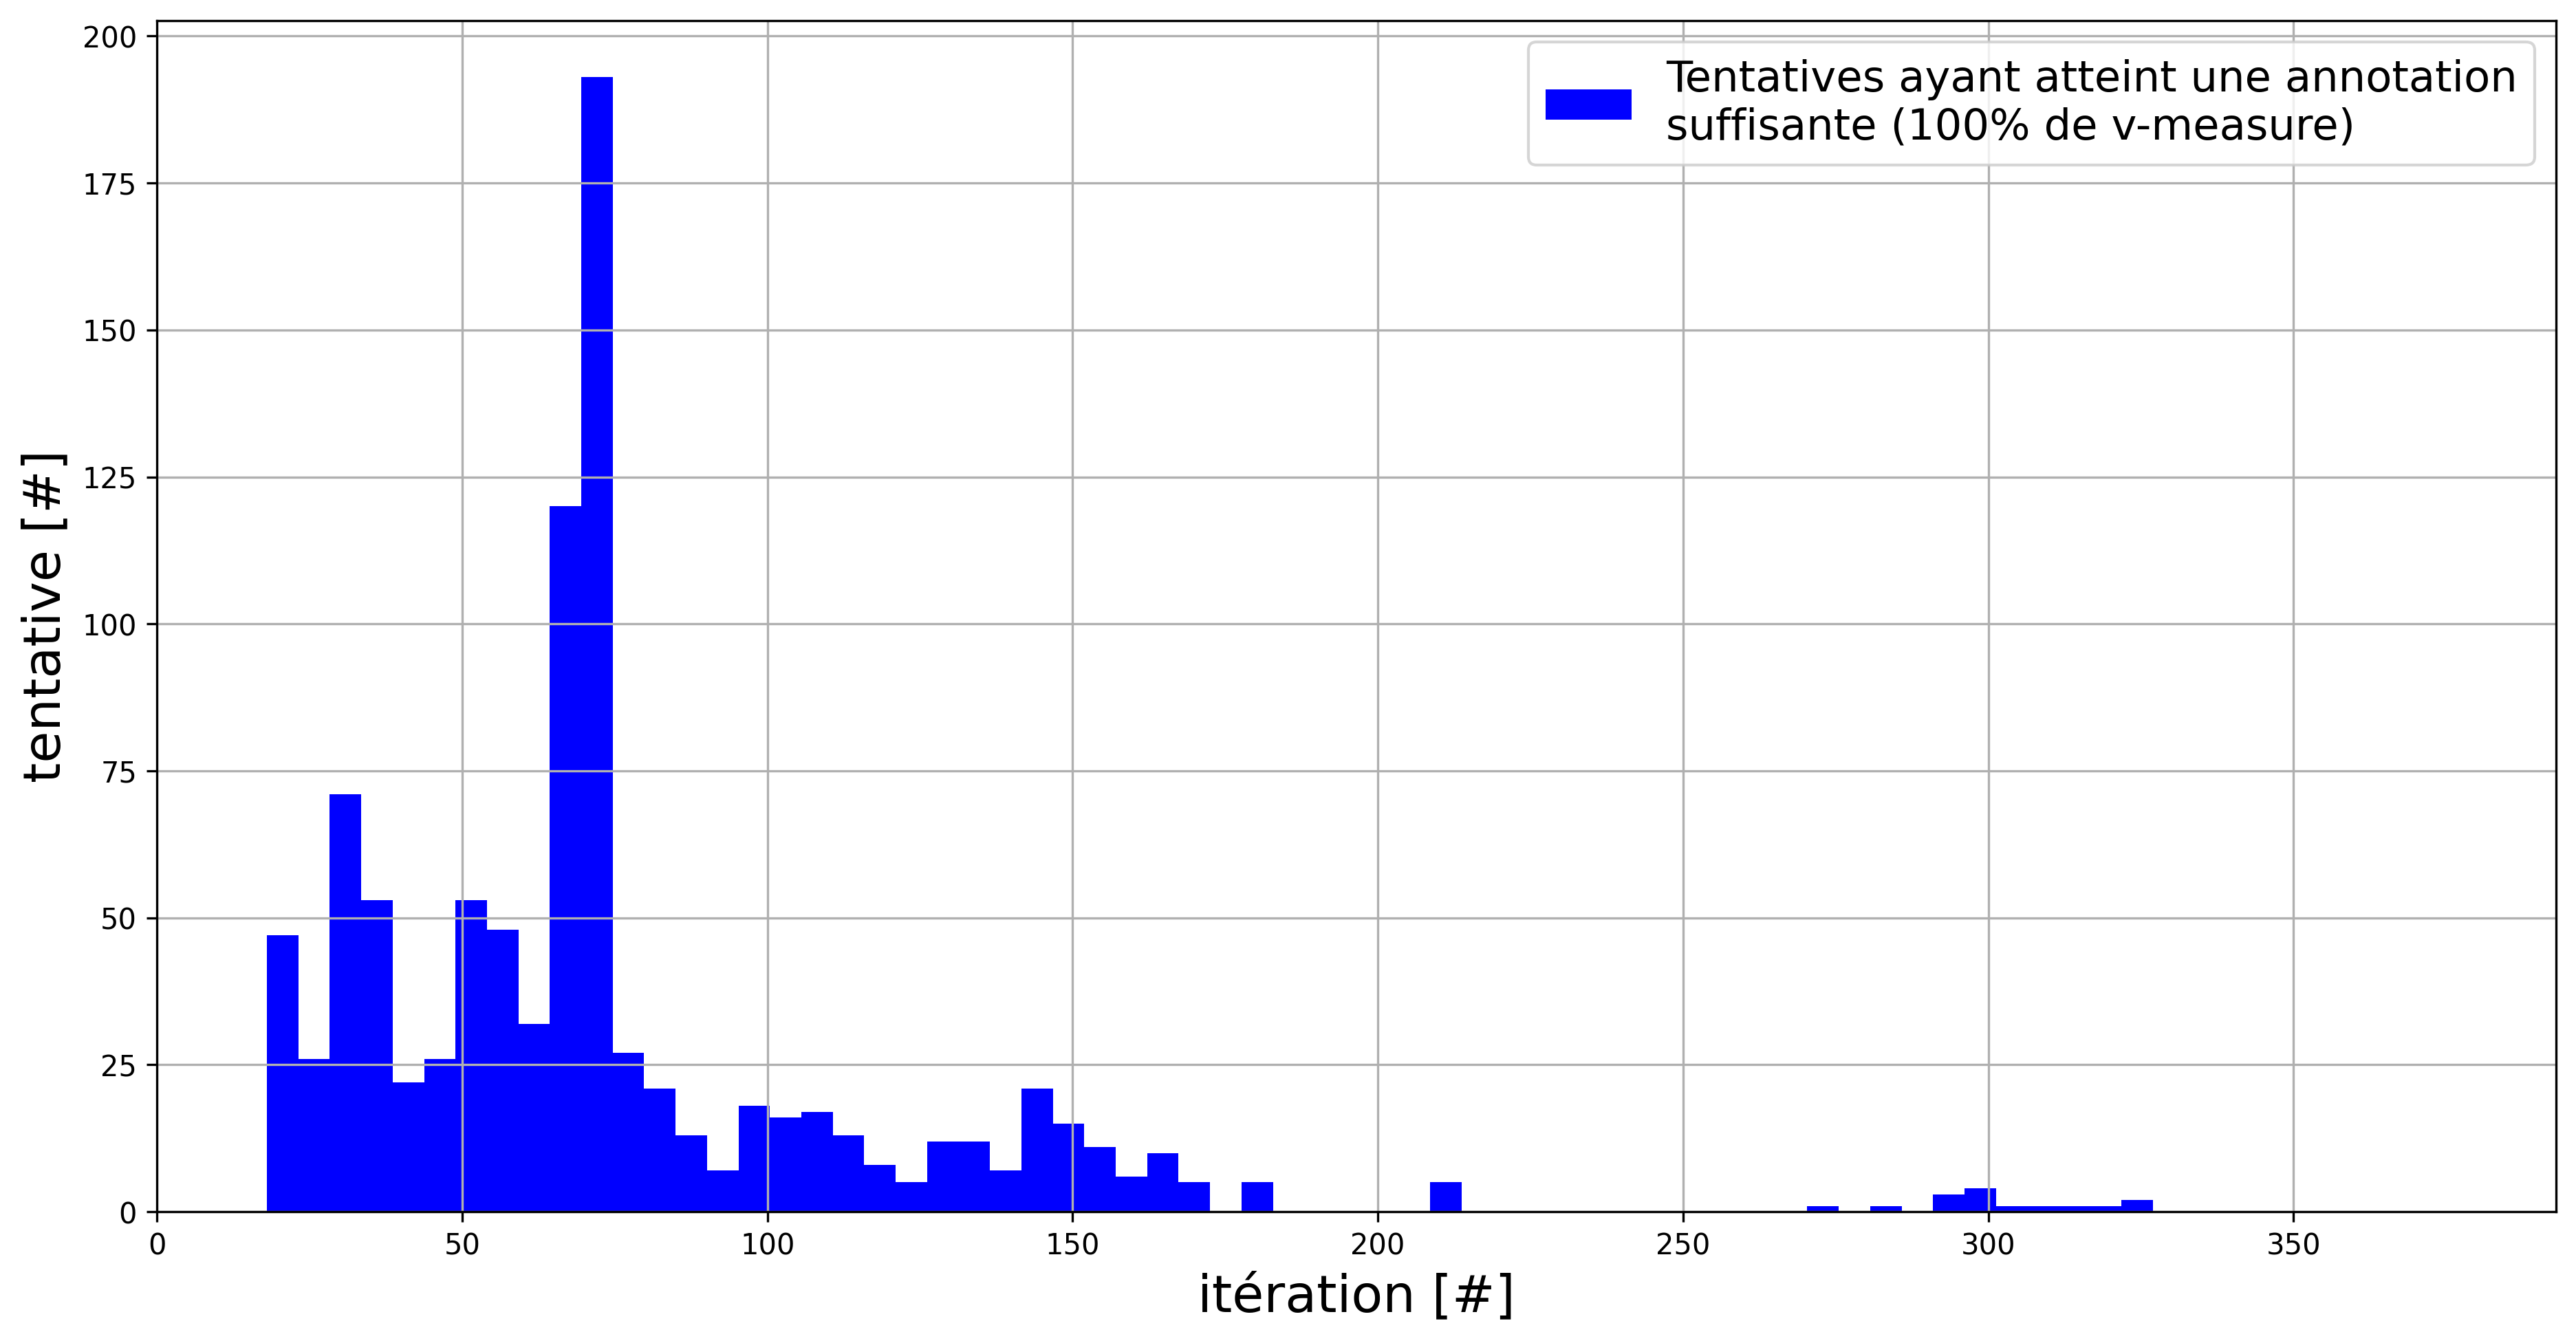
\includegraphics[width=0.7\textwidth]{figures/etude-efficience-histogramme-annotation-suffisante}
				\caption{Répartition des tentatives en fonction de l'itération de la méthode à laquelle elles atteignent le seuil d'une annotation suffisante, c'est-à-dire l'itération à laquelle elles parviennent à \texttt{100}\% de \texttt{v-measure} entre un résultat obtenu et la vérité terrain. L'histogramme est réduit à \texttt{60} pics pour simplifier l'affichage.}
				\label{figure:4.2.1-ETUDE-OPTIMISATION-HISTOGRAMME-ANNOTATION-SUFFISANTE}
			\end{figure}
			%
			Le tableau~\ref{table:4.2.1-ETUDE-OPTIMISATION-ANOVA-ANNOTATION-SUFFISANTE} retranscrit l'influence de chacun des paramètres sur le nombre d'itérations nécessaires pour atteindre une \textbf{annotation suffisante}.
			Les analyses de variance mettent en relief l'effet significatif sur cette convergence du prétraitement (eta-carré: \texttt{0.987}, p-valeur: \(<\) \texttt{\(10^{-3}\)}), de la vectorisation (eta-carré: \texttt{0.991}, p-valeur: \(<\) \texttt{\(10^{-3}\)}), du clustering (eta-carré: \texttt{0.997}, p-valeur: \(<\) \texttt{\(10^{-3}\)}) et de l'échantillonnage (eta-carré: \texttt{0.998}, p-valeur: \(<\) \texttt{\(10^{-3}\)}).
			L'analyse post-hoc de ces effets indique que le meilleur paramétrage moyen pour atteindre une \textbf{annotation suffisante} repose sur la prétraitement \texttt{prep.lemma}, le vectorisation \texttt{vect.tfidf}, le clustering \texttt{clust.kmeans.cop}, et l'échantillonnage \texttt{samp.closest.diff}. La moyenne du nombre d'itération requis pour ce paramétrage est de \texttt{34.60} (écart-type: \texttt{7.44}), soit \texttt{1 730} annotations (écart-type: \texttt{372.00}).
			%
			\begin{table}[!htb]
				\begin{center}
				\begin{tabular}{|c|c|c|c|c|c|c|}
					\hline
					% ENTETE DU TABLEAU
					\multicolumn{2}{|c|}{ \shortstack{Description des \\ facteurs analysés } }
						& \multicolumn{3}{c|}{ \shortstack{ Description \\ statistique } }
						& \multicolumn{2}{c|}{ \shortstack{ Description des \\ tailles d'effets } }
						\tabularnewline
						\hline

					Facteur
						& Niveau 
						& Moyenne
						& Rang
						& SE
						& \texttt{ \( \eta^{2} \) }
						& \texttt{p-valeur}
					\tabularnewline
					\hline
					
					% PRETRAITEMENT
					\multirow{4}{*}{prétraitement}
						& \texttt{prep.lemma}
						& \( 72.86 \)
						& (1)
						& \multirow{4}{*}{ \( 0.32 \) }
						& \multirow{4}{*}{ \( 0.276 \) }
						& \multirow{4}{*}{ \shortstack{ \( < 2e^{-16} \) \\ (\( *** \)) } }
						\tabularnewline
						\cline{2-4}
						
						& \texttt{prep.simple}
						& \( 73.30 \)
						& (2)
						&
						&
						&
						\tabularnewline
						\cline{2-4}
						
						& \texttt{prep.no}
						& \( 75.24 \)
						& (2)
						&
						& 
						&
						\tabularnewline
						\cline{2-4}
						
						& \texttt{prep.filter}
						& \( 83.77 \)
						& (4)
						&
						&
						&
						\tabularnewline
						\hline
					
					% VECTORISATION
					\multirow{2}{*}{vectorisation}
						& \texttt{vect.tfidf}
						& \( 71.16 \)
						& (1)
						& \multirow{2}{*}{ \( 0.36 \) }
						& \multirow{2}{*}{ \( 0.366 \) }
						& \multirow{2}{*}{ \shortstack{\( < 2e^{-16} \) \\ (\( *** \)) } }
						\tabularnewline
						\cline{2-4}
						
						& \texttt{vect.frcorenewsmd}
						& \( 81.43 \)
						& (2)
						&
						&
						&
						\tabularnewline
						\hline
					
					% CLUSTERING
					\multirow{6}{*}{clustering}
						& \texttt{clust.kmeans.cop}
						& \( 62.23 \)
						& (1)
						& \multirow{6}{*}{ \( 0.42 \) }
						& \multirow{6}{*}{ \( 0.700 \) }
						& \multirow{6}{*}{ \shortstack{ \( < 2e^{-16} \) \\ (\( *** \)) } }
						\tabularnewline
						\cline{2-4}
						
						& \texttt{clust.hier.avg}
						& \( 65.13 \)
						& (2)
						&
						&
						&
						\tabularnewline
						\cline{2-4}
						
						& \texttt{clust.hier.sing}
						& \( 75.44 \)
						& (3)
						&
						& 
						&
						\tabularnewline
						\cline{2-4}
						
						& \texttt{clust.hier.ward}
						& \( 80.44 \)
						& (4)
						&
						& 
						&
						\tabularnewline
						\cline{2-4}
						
						& \texttt{clust.hier.comp}
						& \( 81.46 \)
						& (5)
						&
						&
						&
						\tabularnewline
						\cline{2-4}
						
						& \texttt{clust.spec}
						& \( 93.06 \)
						& (6)
						&
						& 
						&
						\tabularnewline
						\hline
					
					% ECHANTILLONNAGE
					\multirow{4}{*}{échantillonnage}
						& \texttt{samp.closest.diff}
						& \( 50.29 \)
						& (1)
						& \multirow{4}{*}{ \( 0.39 \) }
						& \multirow{4}{*}{ \( 0.950 \) }
						& \multirow{4}{*}{ \shortstack{ \( < 2e^{-16} \) \\ (\( *** \)) } }
						\tabularnewline
						\cline{2-4}
						
						& \texttt{samp.random.same}
						& \( 56.38 \)
						& (2)
						&
						&
						&
						\tabularnewline
						\cline{2-4}
						
						& \texttt{samp.random.full}
						& \( 71.95 \)
						& (3)
						&
						& 
						&
						\tabularnewline
						\cline{2-4}
						
						& \texttt{samp.farhtest.same}
						& \( 126.55 \)
						& (4)
						&
						&
						&
						\tabularnewline
						\hline
				\end{tabular}
				\end{center}
				\caption{ANOVA du nombre d'itérations nécessaires pour l'obtention de \texttt{100}\% de v-mesure. Les (\textit{\(*\)}) dénotent le niveau de significativité (\(\alpha=0.05\)). Pour les effets significatifs, les chiffres précisés entre parenthèses dans la colonne \texttt{Moyenne} indiquent le classement des niveaux selon les analyses post-hoc.}
				\label{table:4.2.1-ETUDE-OPTIMISATION-ANOVA-ANNOTATION-SUFFISANTE}
			\end{table}
			
			% Analyse d'une annotation exhaustive.
			Enfin, pour avoir une \textbf{annotation exhaustive} (\textit{annoter toutes les contraintes possibles}), la moyenne des itérations est de \texttt{88.98} (min: \texttt{20}, max: \texttt{394}, écart-type: \texttt{68.21}), soit une moyenne de \texttt{4 431.34} annotations (min: \texttt{1 000}, max: \texttt{19 656}, écart-type: \texttt{3 405.16}).
			La figure~\ref{figure:4.2.1-ETUDE-OPTIMISATION-HISTOGRAMME-ANNOTATION-EXHAUSTIVE} représente la répartition de ces itérations au cours des différentes tentatives.
			On peut noter les deux cas intéressants suivant :
			%
			\begin{itemize}
				\item[\(\bullet\)] Les tentatives les plus rapides furent celles avec un prétraitement des données \texttt{prep.no} ou \texttt{prep.lemma}, une vectorisation des données \texttt{vect.tfidf}, un algorithme de clustering sous contraintes \texttt{clust.hier.comp} ou \texttt{clust.hier.wars}, et un échantillonnage de contraintes \texttt{samp.closest.diff}. Ces tentatives ont requis \texttt{20} itérations, soit \texttt{1 000} annotations, dont \texttt{653} (respectivement \texttt{668}) contraintes \texttt{MUST-LINK}.
				\item[\(\bullet\)] Les tentatives les plus lentes furent celles avec un prétraitement des données \texttt{prep.simple}, une vectorisation des données \texttt{vect.frcorenewsmd}, un clustering sous contraintes \texttt{clust.hier.sing}, et un échantillonnage de contraintes \texttt{samp.closest.diff}. Ces tentatives ont requis \texttt{394} itérations, soit \texttt{19 656} annotations, dont \texttt{682} contraintes \texttt{MUST-LINK}.
			\end{itemize}
			%
			\begin{figure}[!htb]
				\centering
				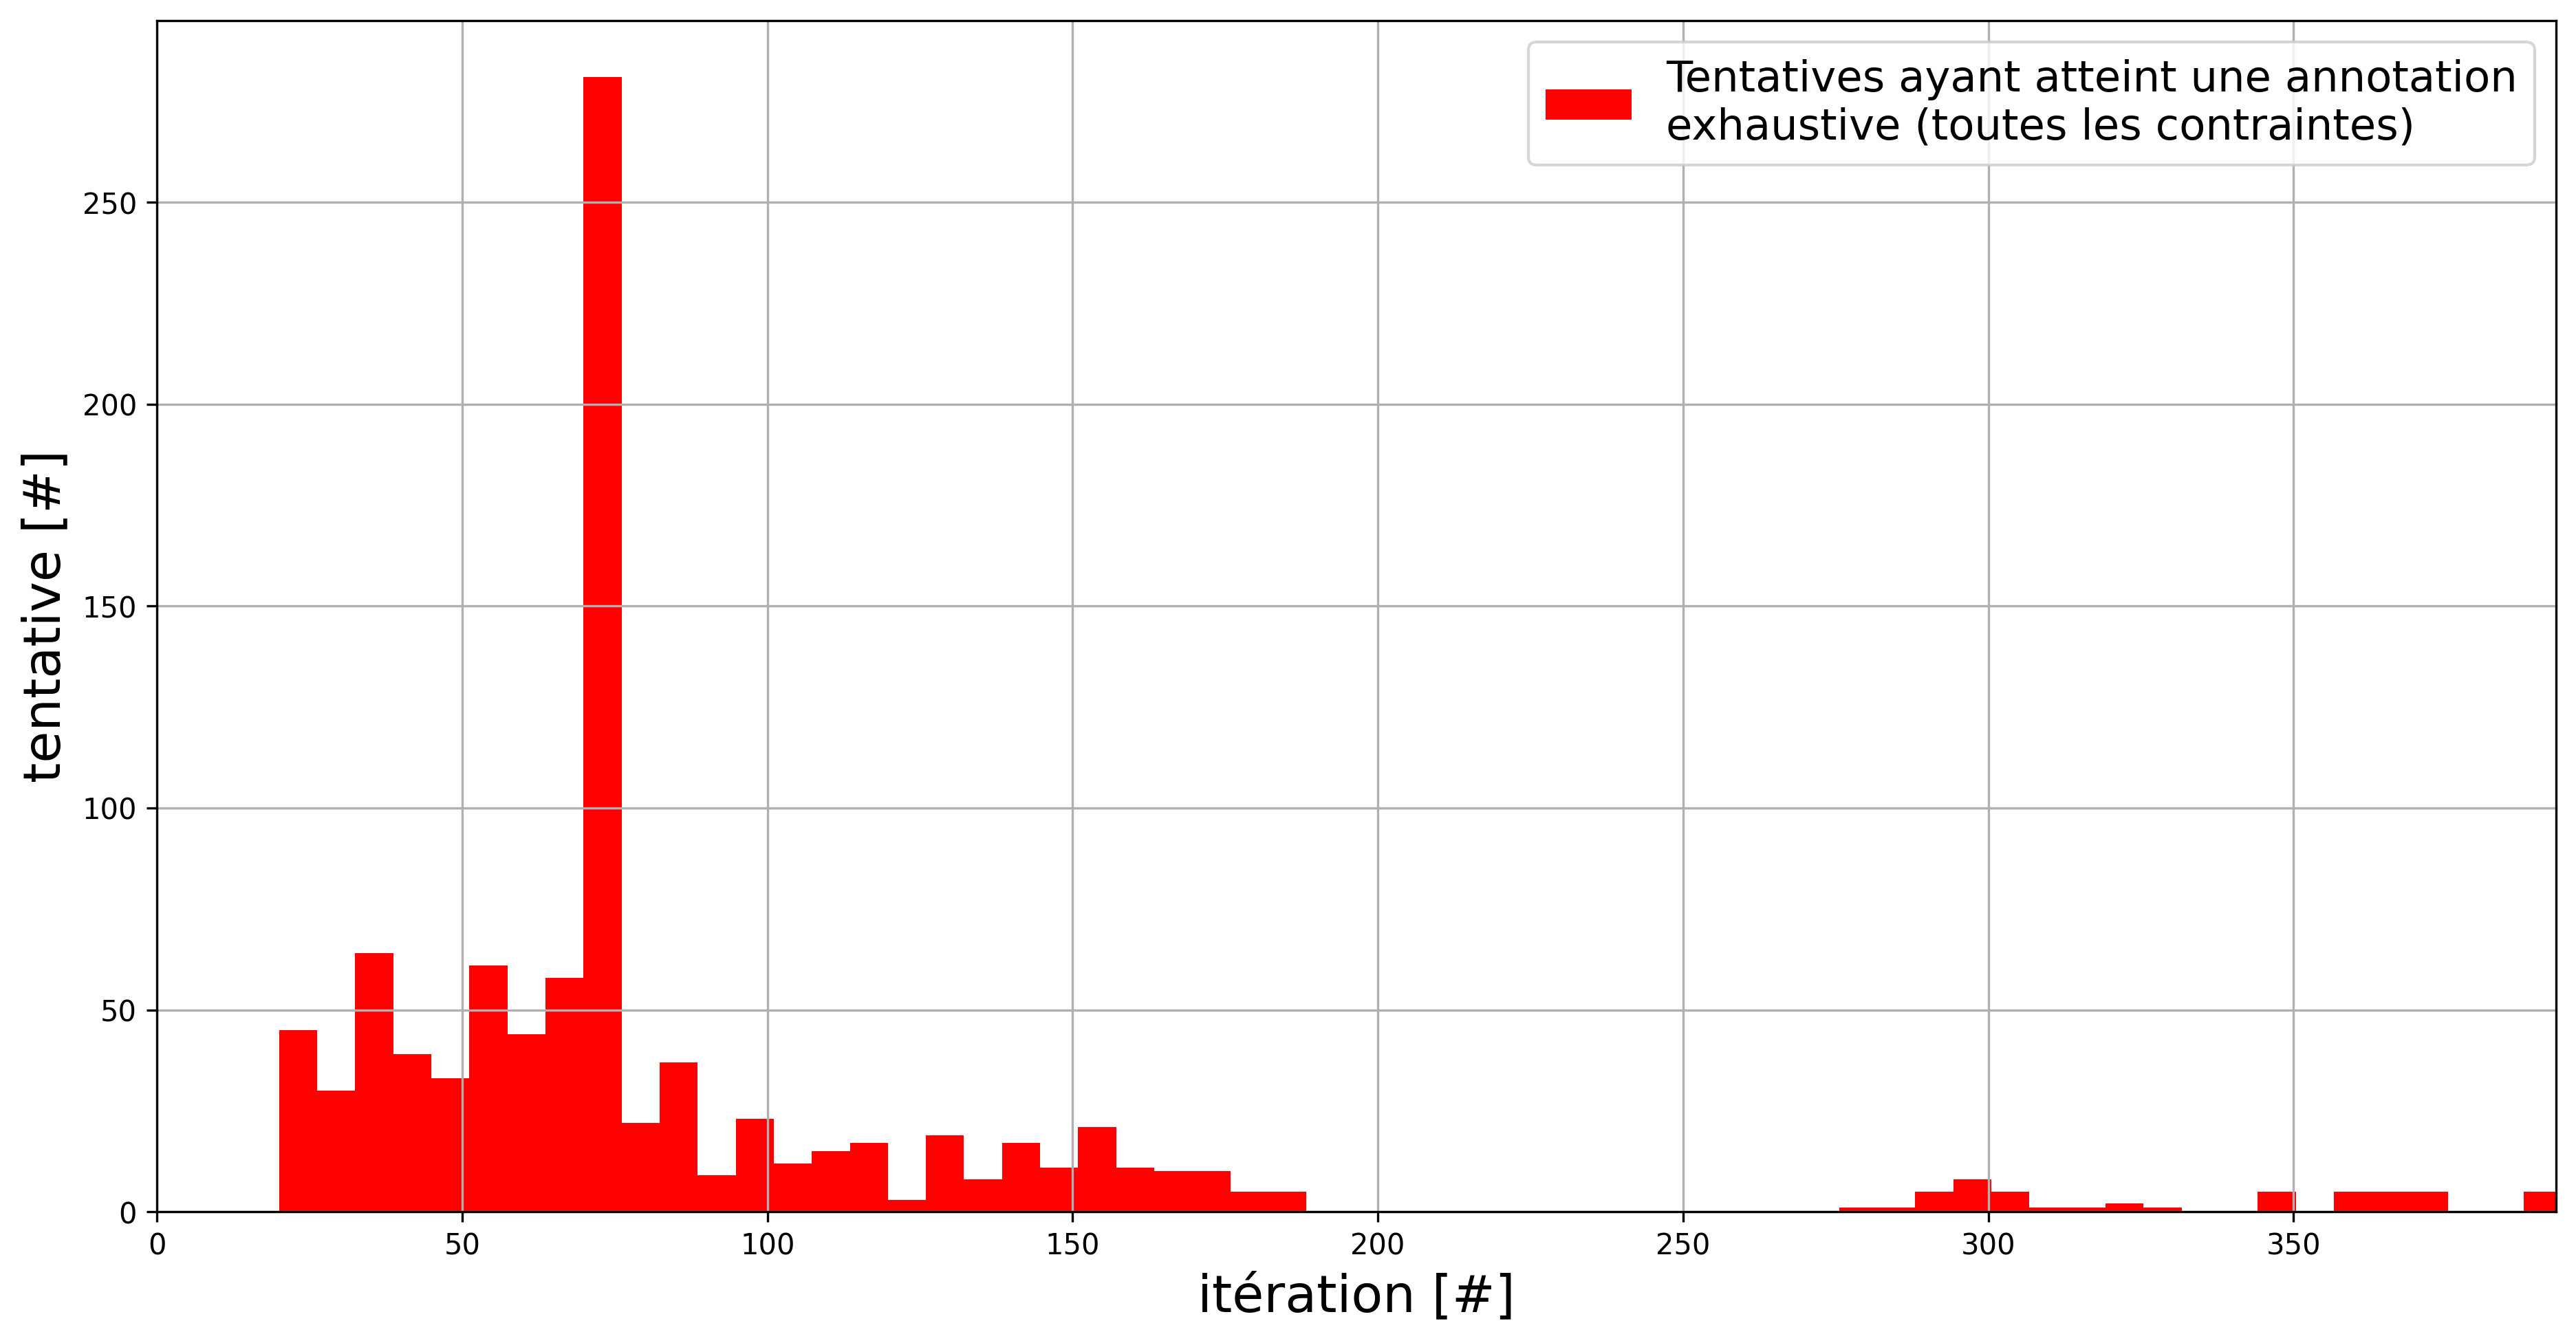
\includegraphics[width=0.7\textwidth]{figures/etude-efficience-histogramme-annotation-exhaustive}
				\caption{Répartition des tentatives en fonction de l'itération de la méthode à laquelle elles atteignent le seuil d'une annotation exhaustive, c'est-à-dire l'itération à laquelle toutes les contraintes possibles entre les données ont été annotées. L'histogramme est réduit à \texttt{60} pics pour simplifier l'affichage.}
				\label{figure:4.2.1-ETUDE-OPTIMISATION-HISTOGRAMME-ANNOTATION-EXHAUSTIVE}
			\end{figure}
			%
			Le tableau~\ref{table:4.2.1-ETUDE-OPTIMISATION-ANOVA-ANNOTATION-EXHAUSTIVE} retranscrit l'influence de chacun des paramètres sur le nombre d'itérations nécessaires pour atteindre une \textbf{annotation exhaustive}.
			Les analyses de variance mettent en relief l'effet significatif sur cette convergence du prétraitement (eta-carré: \texttt{0.909}, p-valeur: \(<\) \texttt{\(10^{-3}\)}), de la vectorisation (eta-carré: \texttt{0.985}, p-valeur: \(<\) \texttt{\(10^{-3}\)}), du clustering (eta-carré: \texttt{0.999}, p-valeur: \(<\) \texttt{\(10^{-3}\)}) et de l'échantillonnage (eta-carré: \texttt{0.997}, p-valeur: \(<\) \texttt{\(10^{-3}\)}).
			L'analyse post-hoc de ces effets indique que le meilleur paramétrage moyen pour atteindre une \textbf{annotation exhaustive} repose sur la prétraitement \texttt{prep.lemma}, le vectorisation \texttt{vect.tfidf}, le clustering \texttt{clust.kmeans.cop}, et l'échantillonnage \texttt{samp.random.same}. La moyenne du nombre d'itération requis pour ce paramétrage est de \texttt{32.60} (écart-type: \texttt{1.14}), soit \texttt{1 630} annotations (écart-type: \texttt{57.00}).
			%
			\begin{table}[!htb]
				\begin{center}
				\begin{tabular}{|c|c|c|c|c|c|c|}
					\hline
					% ENTETE DU TABLEAU
					\multicolumn{2}{|c|}{ \shortstack{Description des \\ facteurs analysés } }
						& \multicolumn{3}{c|}{ \shortstack{ Description \\ statistique } }
						& \multicolumn{2}{c|}{ \shortstack{ Description des \\ tailles d'effets } }
						\tabularnewline
						\hline

					Facteur
						& Niveau 
						& Moyenne
						& Rang
						& SE
						& \texttt{ \( \eta^{2} \) }
						& \texttt{p-valeur}
					\tabularnewline
					\hline
					
					% PRETRAITEMENT
					\multirow{4}{*}{prétraitement}
						& \texttt{prep.lemma}
						& \( 85.89 \)
						& (1)
						& \multirow{4}{*}{ \( 0.42 \) }
						& \multirow{4}{*}{ \( 0.052 \) }
						& \multirow{4}{*}{ \shortstack{ \( < 2e^{-16} \) \\ (\( *** \)) } }
						\tabularnewline
						\cline{2-4}
						
						& \texttt{prep.filter}
						& \( 89.55 \)
						& (2)
						&
						&
						&
						\tabularnewline
						\cline{2-4}
						
						& \texttt{prep.simple}
						& \( 89.64 \)
						& (2)
						&
						& 
						&
						\tabularnewline
						\cline{2-4}
						
						& \texttt{prep.no}
						& \( 90.81 \)
						& (4)
						&
						&
						&
						\tabularnewline
						\hline
					
					% VECTORISATION
					\multirow{2}{*}{vectorisation}
						& \texttt{vect.tfidf}
						& \( 85.50 \)
						& (1)
						& \multirow{2}{*}{ \( 0.39 \) }
						& \multirow{2}{*}{ \( 0.165 \) }
						& \multirow{2}{*}{ \shortstack{\( < 2e^{-16} \) \\ (\( *** \)) } }
						\tabularnewline
						\cline{2-4}
						
						& \texttt{vect.frcorenewsmd}
						& \( 92.46 \)
						& (2)
						&
						&
						&
						\tabularnewline
						\hline
					
					% CLUSTERING
					\multirow{6}{*}{clustering}
						& \texttt{clust.kmeans.cop}
						& \( 64.99 \)
						& (1)
						& \multirow{6}{*}{ \( 0.39 \) }
						& \multirow{6}{*}{ \( 0.894 \) }
						& \multirow{6}{*}{ \shortstack{ \( < 2e^{-16} \) \\ (\( *** \)) } }
						\tabularnewline
						\cline{2-4}
						
						& \texttt{clust.hier.avg}
						& \( 78.54 \)
						& (2)
						&
						&
						&
						\tabularnewline
						\cline{2-4}
						
						& \texttt{clust.hier.ward}
						& \( 81.31 \)
						& (3)
						&
						& 
						&
						\tabularnewline
						\cline{2-4}
						
						& \texttt{clust.hier.comp}
						& \( 82.49 \)
						& (3)
						&
						& 
						&
						\tabularnewline
						\cline{2-4}
						
						& \texttt{clust.spec}
						& \( 93.78 \)
						& (5)
						&
						&
						&
						\tabularnewline
						\cline{2-4}
						
						& \texttt{clust.hier.comp}
						& \( 132.75 \)
						& (6)
						&
						& 
						&
						\tabularnewline
						\hline
					
					% ECHANTILLONNAGE
					\multirow{4}{*}{échantillonnage}
						& \texttt{samp.random.same}
						& \( 57.23 \)
						& (1)
						& \multirow{4}{*}{ \( 0.42 \) }
						& \multirow{4}{*}{ \( 0.930 \) }
						& \multirow{4}{*}{ \shortstack{ \( < 2e^{-16} \) \\ (\( *** \)) } }
						\tabularnewline
						\cline{2-4}
						
						& \texttt{samp.random.full}
						& \( 72.80 \)
						& (2)
						&
						&
						&
						\tabularnewline
						\cline{2-4}
						
						& \texttt{samp.closest.diff}
						& \( 98.38 \)
						& (3)
						&
						& 
						&
						\tabularnewline
						\cline{2-4}
						
						& \texttt{samp.farhtest.same}
						& \( 132.75 \)
						& (4)
						&
						&
						&
						\tabularnewline
						\hline
				\end{tabular}
				\end{center}
				\caption{ANOVA du nombre d'itérations nécessaires pour annoter toutes les contraintes possibles. Les (\textit{\(*\)}) dénotent le niveau de significativité (\(\alpha=0.05\)). Pour les effets significatifs, les chiffres précisés entre parenthèses dans la colonne \texttt{Moyenne} indiquent le classement des niveaux selon les analyses post-hoc.}
				\label{table:4.2.1-ETUDE-OPTIMISATION-ANOVA-ANNOTATION-EXHAUSTIVE}
			\end{table}
		
		
			% Graphe d'évolution de la v-measure moyenne, min et max.
			La figure~\ref{figure:4.2.1-ETUDE-OPTIMISATION-EVOLUTION-PAR-FACTEURS} représente les évolutions moyennes de la \texttt{v-measure} du clustering en fonction du nombre d'itération de la méthode pour les différentes valeurs des facteurs analysés (prétraitement en haut à gauche, vectorisation en haut à droite, clustering en bas à gauche, échantillonnage en bas à droite).
			La figure~\ref{figure:4.2.1-ETUDE-OPTIMISATION-EVOLUTION-MEILLEUR-PARAMETRAGE} représente cette même évolution pour les meilleurs paramétrages moyens destinés à atteindre les trois seuils d'annotation définis (partiel, suffisant, exhaustif).
			%
			\begin{figure}[!htb]
				\centering
				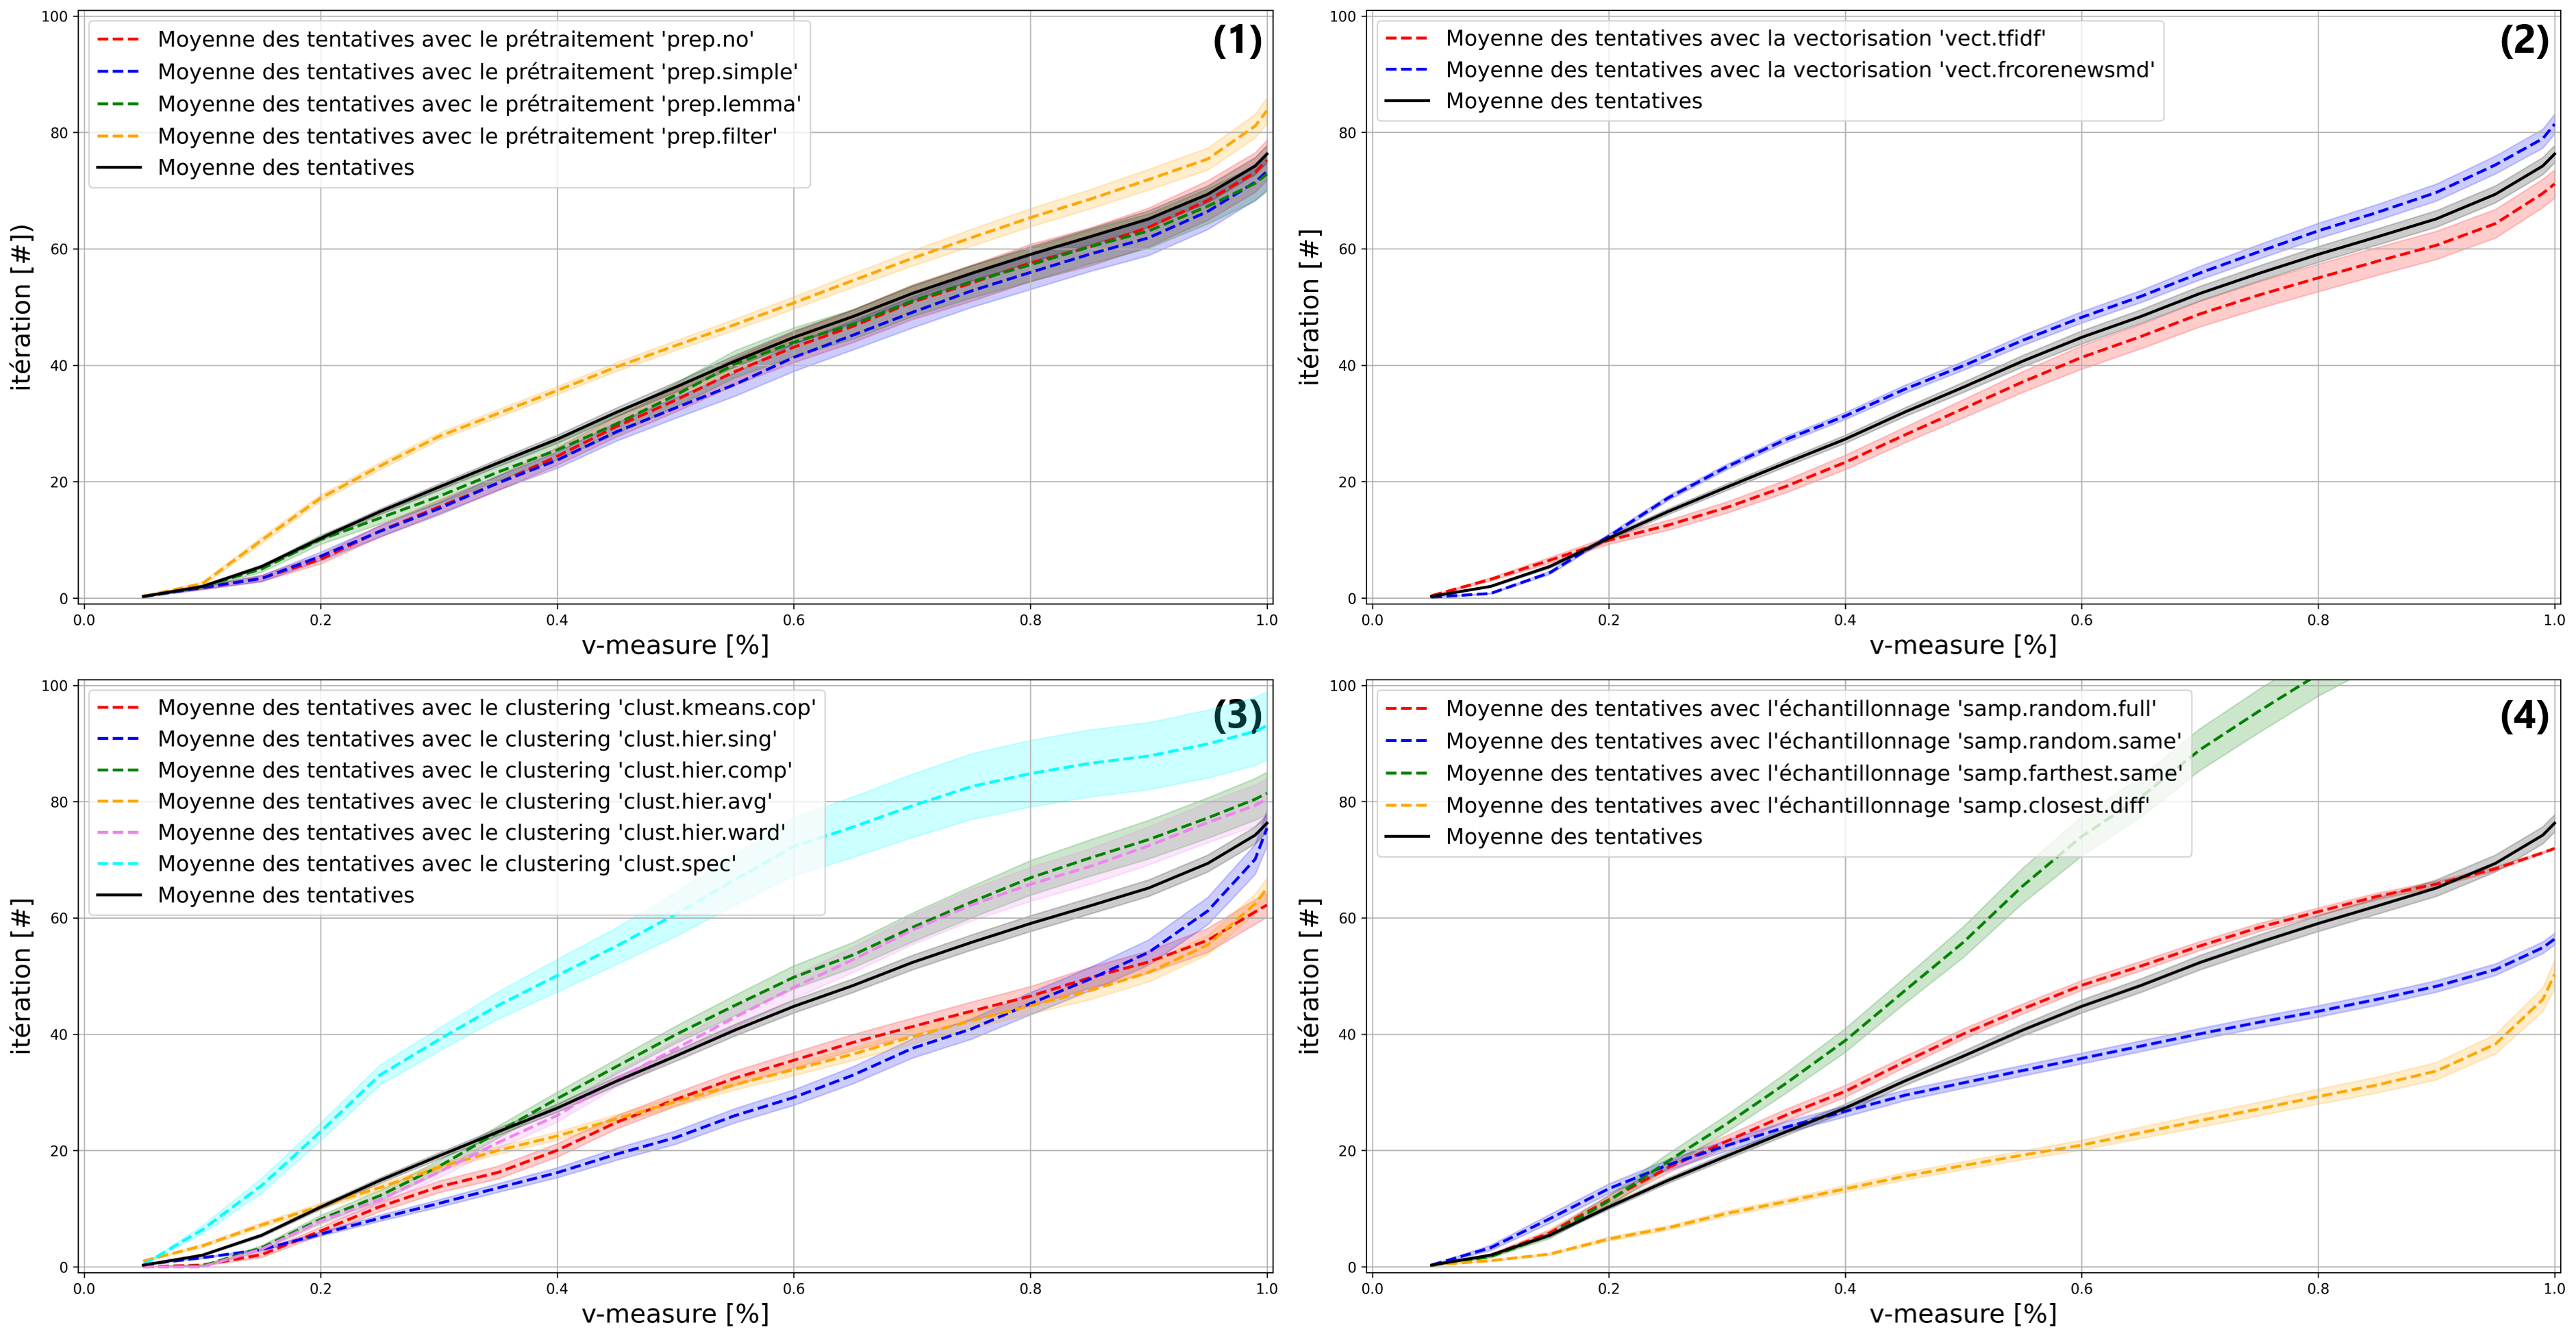
\includegraphics[width=\textwidth]{figures/etude-efficience-evolution-moyenne-par-vmeasure-par-facteur}
				\caption{Évolution des moyennes du nombre d'itérations nécessaire de la méthode de \textit{clustering} interactif pour obtenir un seuil défini de \texttt{v-measure} entre un résultat obtenu et la vérité terrain, moyennes réalisées sur les différentes valeurs que peuvent prendre les facteurs analysés et affichées par facteur : \textbf{(1)} prétraitement, \textbf{(2)} vectorisation, \textbf{(3)} clustering et \textbf{(4)} échantillonnage. Le seuil d'annotation exhaustive (annoter toutes les contraintes possibles) n'étant pas exprimé en terme de \texttt{v-measure}, ce seuil n'est pas affiché ici.}
				\label{figure:4.2.1-ETUDE-OPTIMISATION-EVOLUTION-PAR-FACTEURS}
			\end{figure}
			%
			\begin{figure}[!htb]
				\centering
				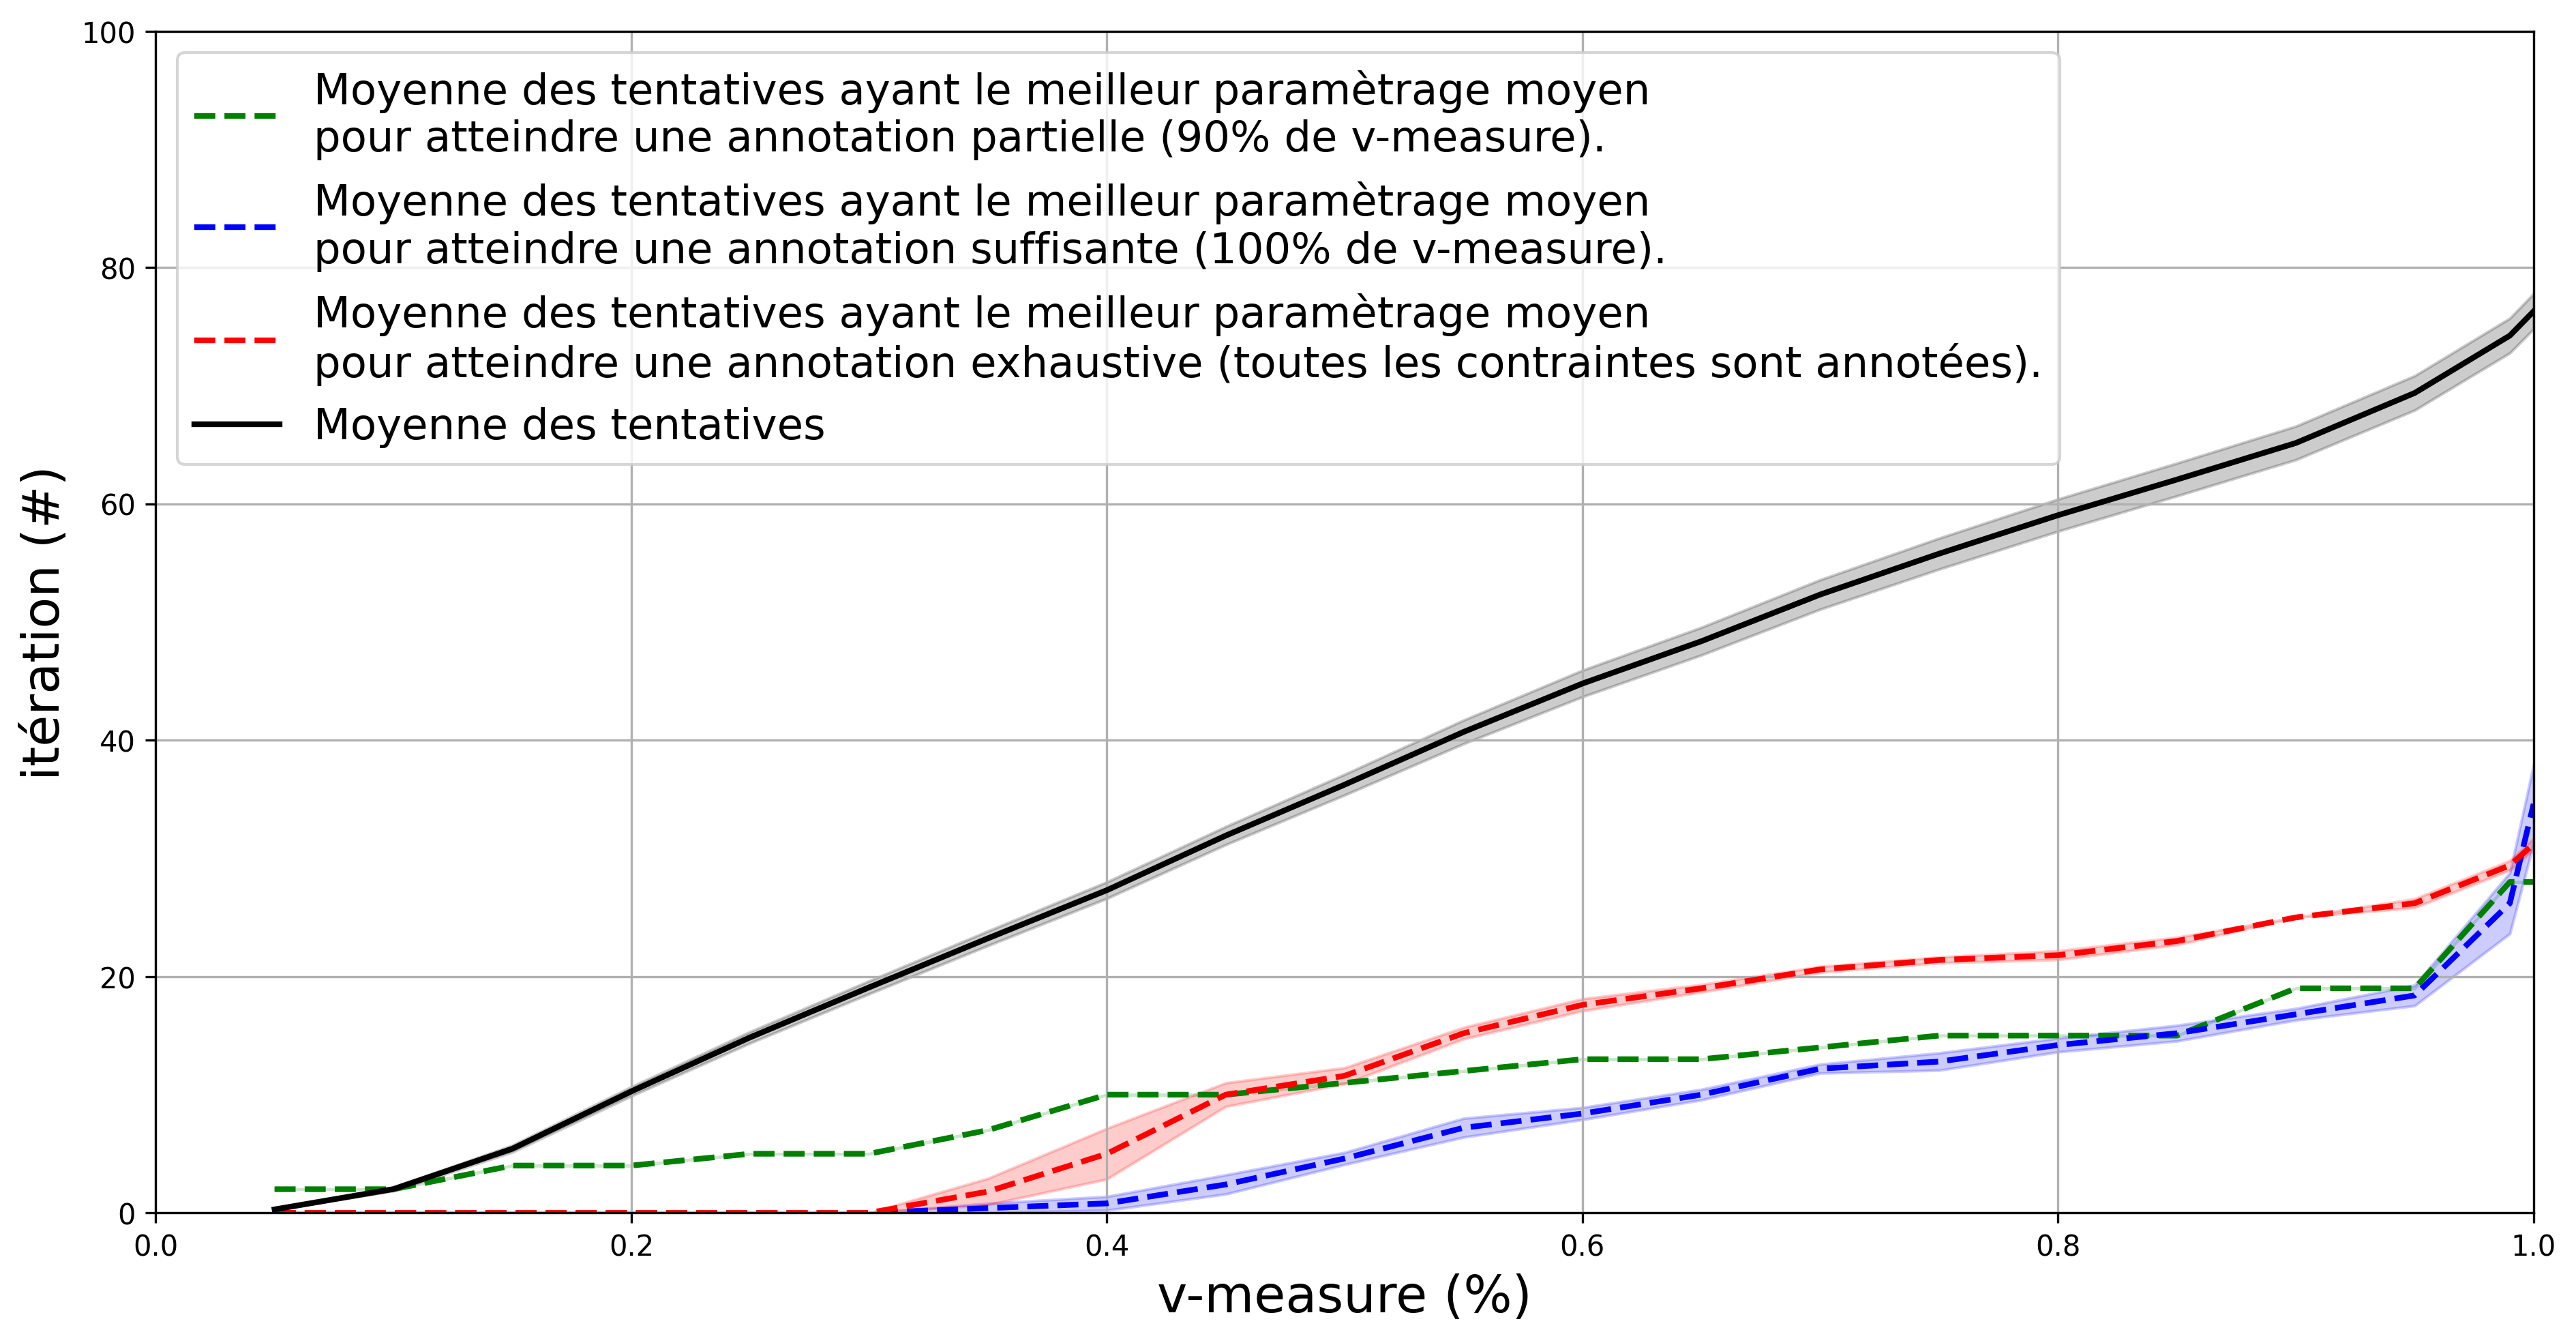
\includegraphics[width=0.8\textwidth]{figures/etude-efficience-evolution-moyenne-5best-par-vmeasure}
				\caption{Évolution des moyennes du nombre d'itérations nécessaire de la méthode de \textit{clustering} interactif pour obtenu un seuil défini de \texttt{v-measure} entre un résultat obtenu et la vérité terrain, moyennes réalisées sur les différentes seuils d'annotations étudiés : l'annotation partielle (\textit{atteindre une \texttt{v-measure} de \texttt{90}\%}), l'annotation suffisante (\textit{atteindre une \texttt{v-measure} de \texttt{100}\%}) et l'annotation exhaustive (\textit{annoter toutes les contraintes possibles}).}
				\label{figure:4.2.1-ETUDE-OPTIMISATION-EVOLUTION-MEILLEUR-PARAMETRAGE}
			\end{figure}

		%%% Discussion
		\subsubsection{Discussion}

			% Rappel de l'objectif : être efficient.
			L'objectif de l'étude est de trouver une implémentation "efficiente" du \textit{clustering} interactif permettant d'obtenir une base d'apprentissage correctement annotée en un minimum d'annotation.
			Pour trouver si une telle implémentation existe et quels en sont les paramètres optimaux, nous avons analysé l'impact de différentes paramétrages sur les tâches principales de la méthode (\textbf{prétraitement}, \textbf{vectorisation}, \textbf{clustering sous contraintes}, \textbf{échantillonnage}) en nous basant sur des simulations d'annotation d'un jeu de données.
			
			% Première remarque : Choix d'un seuil à 90\% de v-measure.
			Dans l'optique d'être efficient, nous excluons le désir d'annoter \textbf{exhaustivement} le jeu de données car la charge de travail estimée est trop importante.
			(cf. discussion de la section~\ref{section:4.1-HYPOTHESE-EFFICACITE} (hypothèse d'efficacité))
			Nous préférons donc nous concentrer sur deux seuils d'annotation plus réalistes : celui d'une \textbf{annotation partielle} (atteindre \texttt{90}\% de \texttt{v-measure} avec la vérité terrain) et celui d'une \textbf{annotation suffisante} (atteindre \texttt{100}\% de \texttt{v-measure} avec la vérité terrain en un minimum de contraintes). 
			
			% Meilleur paramétrage.
			L'étude réalisée met en avant l'impact significatif des quatre tâches principales (\textbf{prétraitement}\todo{remarque sur la valeur de eta2}, \textbf{vectorisation}\todo{remarque sur la valeur de eta2}, \textbf{clustering sous contraintes}, \textbf{échantillonnage}) sur la vitesse de convergence de la méthode pour atteindre les seuils définis de \texttt{90}\% et \texttt{100}\% de \texttt{v-measure}. Il existe donc bien un paramétrage permettant d'optimiser l'implémentation proposée et de réduire le nombre de contraintes nécessaires à annoter :
			\begin{enumerate}
				\item pour une \textbf{annotation partielle} (\texttt{90}\% de \texttt{v-measure}), le meilleur paramétrage moyen est constitué du prétraitement simple (\texttt{prep.simple}), de la vectorisation TF-IDF (\texttt{vect.tfidf}), du clustering hiérarchique à lien moyen (\texttt{clust.hier.avg}) et de l'échantillonnage des données les plus proches dans des clusters différents (\texttt{sampl.closest.diff}). Avec ce paramétrage, il faut en moyenne \texttt{950} annotations de contraintes pour obtenir une \texttt{v-measure} de \texttt{90}\% ;
				\item pour une \textbf{annotation suffisante} (\texttt{100}\% de \texttt{v-measure}), le meilleur paramétrage moyen est constitué du prétraitement avec lemmatisation (\texttt{prep.lemma}), de la vectorisation TF-IDF (\texttt{vect.tfidf}), du clustering KMeans (\texttt{clust.kmeans.cop}) et de l'échantillonnage des données les plus proches dans des clusters différents (\texttt{sampl.closest.diff}). Avec ce paramétrage, il faut en moyenne \texttt{1 750} annotations de contraintes pour obtenir une \texttt{v-measure} de \texttt{100}\% ;
				\item le cas d'une \textbf{annotation exhaustive} (annoter toutes les contraintes possibles sur les données) n'est pas explicité ici mais peut se déduire des résultats décrits plus haut.
			\end{enumerate}


			%%% Avantages.
			Ainsi, cette étude permet de répondre à certaines limites discutées dans la section~\ref{section:4.1-HYPOTHESE-EFFICACITE} (hypothèse d'efficacité). 
			
			% Avantage 1: Optimisation du nombre de contraintes.
			En effet, l'optimisation des paramètres de l'implémentation du \textit{clustering} interactif permet de réduire considérablement le nombre de contraintes nécessaires pour obtenir une base d'apprentissage exploitable.
			En nous basant sur le tableau~\ref{table:4.1.1-ETUDE-CONVERGENCE-EVOLUTION} de l'étude de convergence, et dans le cadre de l'annotation d'un jeu de \texttt{500} données, nous sommes passé d'un paramétrage moyen nécessitant \texttt{3 750} (respectivement \texttt{10 000}) contraintes à un paramétrage optimisé ne nécessitant que \texttt{950} (respectivement \texttt{1 750}) contraintes pour atteindre un seuil de \texttt{90}\% (respectivement \texttt{100}\%) \texttt{v-measure}.
			L'ordre de grandeur de la charge de travail demandée aux annotateurs est donc située entre \texttt{2} et \texttt{4} fois la taille du jeu de données.
			
			% Avantage 2: La méthode devient réaliste !
			En considérant que les annotations sont binaires et demandent a priori une charge mental plus faible que les annotations par attribution de label ("\textit{les données sont-elles similaires ?}" vs "\textit{quel est l'étiquette de cette donnée ?}"), nous pouvons conclure que la charge totale nécessaire à l'annotation avec une méthodologie basée sur le \textit{clustering} interactif est comparable à celles des méthodes traditionnelles.
			De plus, cette méthode ne demande pas de formalisation concrète de la structure de données à annoter pour faire émerger une base d'apprentissage au cours des itérations, donc le \textit{clustering} interactif devient une méthode d'annotation adaptée à l'activité des annotateurs.
			
			%%% Limites.
			Néanmoins, quelques pistes sont encore à explorer pour compléter cette analyse d'efficience.
			
			% Limite 1 : Coût temporel.
			D'une part, une étude de coût est à réaliser pour trancher le choix de paramètre optimaux réalistes. En effet, il est intéressant d'étudier le coût machine (temps CPU utilisé) et le coût humain (temps d'annotation) afin d'affiner les choix techniques et de compléter les arguments sur l'utilisation en situation réelle d'une méthodologie d'annotation basée sur le \textit{clustering} interactif.
			Cet aspect sera traité dans la section~\ref{section:4.3-HYPOTHESE-COUTS} (hypothèse des coûts).
			
			% Limite 2 : Valeur métier de ce 90\% (pas de vérité terrain en pratique).
			D'autre part, l'étude réalisée se base sur des seuils de performance par rapport à une vérité terrain.
			Or en situation réelle, cette comparaison avec la vérité terrain n'est pas possible car elle est précisément en cours de conception (la base d'apprentissage finale devant être la vérité terrain).
			De plus, un tel score n'est pas le plus explicite pour pour un expert métier pour qui un score de \texttt{v-measure} n'est pas révélateur de la pertinence métier de la segmentation proposée des données.
			Il manque donc une stratégie d'évaluation de pertinence de la base d'apprentissage en cours de construction et de la suffisance des annotations réalisées pour faire refléter la vision de l'annotateur dans le résultat.
			Cet aspect sera traité dans la section~\ref{section:4.4-HYPOTHESE-PERTINENCE} (hypothèse de pertinence).
			
			% Limite 3 : Expert métier parfait ==> simuler les erreurs.
			Pour finir, comme pour l'étude de convergence réalisé en section~\ref{section:4.1-HYPOTHESE-EFFICACITE}, nous avons supposé dans cette étude que l'annotateur est un expert métier connaissant parfaitement le domaine traité.
			Cette hypothèse forte n'est a priori pas valable en situation réelle : En effet, des erreurs d'annotations peuvent intervenir (ambiguïtés sur les données, méconnaissance du domaine, erreurs d'inattention, différence d'opinions entre annotateurs, ...), ce qui peut entraîner des divergences ou des incohérences dans la construction de la base d'apprentissage.
			Il semble donc nécessaire d'étudier les impacts de ces incohérences, ainsi que de proposer une méthode pour les prévenir ou les corriger.
			Cet aspect sera traité à la fin de ce chapitre dans la section~\ref{section:4.6-HYPOTHESE-ROBUSTESSE} (hypothèse de robustesse).